\documentclass[12pt, a4paper]{article}
\usepackage[utf8]{inputenc}

\usepackage{graphicx}

\usepackage{geometry}

\usepackage{multicol}
\usepackage{listings}


\usepackage{amsmath}
\usepackage{amsfonts}
\usepackage{amssymb}

\geometry{margin=0.6in}


\setlength{\parindent}{0em}
\setlength{\parskip}{1em}

\title{Calcolatori}

\begin{document}

\section{INTRODUZIONE}
\subsection{Astrazioni}
Per isolare i vari livelli di un computer (hardware, kernel, SO), ogni strato fornisce delle interfacce (o set di istruzioni) con la quale interagire al livello sottostante.
Le più importanti sono:
\begin{itemize}
    \item ISA (Instruction Set Architecture) $\rightarrow$ insieme istruzioni macchina
    \item ABI (Application Binary Interface) $\rightarrow$ interfaccia delle applicazioni
\end{itemize}

\subsection{prestazioni}
Le prestazioni si misurano con il \textbf{tempo di esecuzione di un programma} che è composto da 3 variabili:
\textbf{numero di istruzioni}, \textbf{cicli di clock per istruzione} e \textbf{frequenza di clock}
\begin{center}
    tempo di CPU = $\frac{numero\ istruzioni\ \times \ CPI}{frequenza\ di\ clock}$
\end{center}

\subsection{ISA}
 - influisce direttamente sul tempo di cpu (un isa è progettata per frequenze di clock più spinte, è esplicitato il numero di cicli per un'instruzione, e il numero di istruzioni stesso per compiere un'operazione)
 le ISA che affronteremo:
 \begin{itemize}
    \item RISC-V (RISC): cloud computing e sistemi embedded
    \item Intel (CISC): PC
    \item ARM (A-RISC): embedded e mobile
 \end{itemize}


\section{ARITMETICA DEI CALCOLATORI}

\subsection{Basi}
 L'aritmetica nei calcolatori viene fatta su base binaria, quindi bisogna eseguire delle conversioni da una base all'altra.
 per un passaggio da decimale a binario, prendo il numero in decimale e calcolo ricorsivamente il modulo di 2, da qui tengo la parte il resto.
 Quando arrivo a 1, il mio numero in binario saranno i resti letti al contrario.
 
 L'addizione in decimale e binario rimane uguale, mentre le moltiplicazioni seguono questo algoritmo: per ogni 0 del moltiplicatore
 mi sposto di un posto a sinistra, mentre con un 1 copio il moltiplicando. Alla fine addiziono tutto.

\subsection{Codifica}
\subsubsection{Numeri negativi}
Esistono 3 metodi per rappresentare i numeri negativi: \textbf{modulo e segno}, \textbf{complemento a 1}, \textbf{complemento a 2}. 
Con tutti questi metodi, il bit più a sinistra rappresenta il segno

\textbf{modulo e segno:} il più semplice, con il bit più a sinistra rappresenta il segno (1 per -, 0 per +)

\textbf{complemento a 1:} un numero positivo viene rappresento come valore assoluto, mentre uno negativo
 lo rappresento con complimento a 1. \\
    I metodi del complemento sono 2:\\
    - cambio tutti i bit da 1 a 0 e da 0 a 1\\
    - sottraggo il numero a un numero della stessa lunghezza con tutti i bit a 1 
    (11111 - 00101 = 11010)
   
\textbf{Somma e sottrazione con complemento a 1:}
    i numeri negativi li rappresento con complemento a 1 e poi sommo i 2 numeri.Il riporto sul bit più significativo
    lo sommo al risultato. 
    \begin{center}
         6-3 $\rightarrow$ 6 + (-3) $\rightarrow$ 00110 + 11100 $\rightarrow$ 00010 con riporto di 1 $\rightarrow$
         00010 + 1 = 00011 = 3
    \end{center}

\textbf{complemento a 2:}
per eseguire un complemento a 2 si possono usare 3 metodi:
\\ - metodo 1: dato un numero trovo il primo bit a 1 partendo da destra, poi eseguo il complemento a 1 per tutti i bit successivi
\\ - metodo 2: eseguo il complemento a uno del numero, e poi addiziono 1
\\ - metodo 3: prendo il numero con primo bit di sinistra a 1 e resto a zero e di lunghezza pari al numero che ci interessa, infine sottraggo quest'ultimo

Il complemento a 2 risulta più conveniente per le somme, la codifica dello zero è unica e nell'operazione inversa, infatto per eseguire quest'ultima
si osserva il primo bit. Se è pari a 0, allora converto normalmente, se no eseguo il complemento a 2 e sommo 1, poi converto in base 10
\\Il vantaggio con il complemento a 2 si guadagna un valore negativo. Sfortunatamento però si posson oanche generare degli overflow.
Bisogna sempre controllare se da somma di positiva risulta in negativo o se da somma di negativi risulta un positivo
 


\subsubsection{Rappresentazione numeri reali}
\textbf{virgola fissa}
  - si dedica una parte della stringa di bit come parte intera e parte frazionaria
  - genericamente trattiamo il numero come intero e poi moltiplichiamo per -n (dove n rappresenta le cifre decimali)
  - non ci sono errori di approsimazione, ma risulta difficile gestire numeri particolarmente grandi o piccoli
  - per la conversione della parte decimale moltiplico per 2 e considero le parti intere

\textbf{virgola mobile}
  - un numero reale viene suddiviso come mantissa ed esponente
\newpage
\subsection{Codifica del testo}
\subsubsection{ASCII}
\marginpar{NB: 0x denota l'utilizzo di codifica esadecimale}
Per la codifica del testo si usa l'Ascii (American Standard Code for Information Interchange).
Ci sono 2 versioni: ASCII
e ex-ASCII (o ASCII extendend). La differenza tra i due è che il primo uso 7 bit per la codifica, mentre il secondo usa anche il bit significativo
Il bit significativo del ex-ASCII, espande nuove lettere in base al codice del linguaggio 
(8859-1 - caratteri europa occidentale, 8859-5 - cirillico,...). L'extendend inoltre può causare problemi di condivisione data
la sua dipendenza dal codice dei caratteri.\\
Per ulteriori caratteri si utilizza l'unicode o UTF, nelle vari versioni a 32,16 o 8 bit. l'UTF-8 è compatibile con ASCII

\newpage
\section{Reti logiche}
- nei circuiti elettronici, i transistor hanno 2 livelli: uno alto per 1 e uno basso per 0
- le reti logiche sono circuiti che dati valori logici in entrata, ne forniscono altri un uscita
 - possono essere combinatorie, cioé senza memoria e l'uscita dipende solo dal valore in ingresso
 - possono essere sequenziali, cioé hanno memoria e l'uscita dipende anche dai precedenti ingressi
- tabella di verità, espone gli uotput di tutte le combinazioni di input

\subsection{Algebra di Boole}
L'algebra di boole viene utilizzata per le operazioni logiche. gli operatori di base sono l'AND ($\cdot$), l'OR (+) e il NOT ($\overline{A}$)
Come l'algebra matematica, l'algebra di boole possiede delle proprietà
\begin{itemize}
  \item A+0=A, A$\cdot$1=A (identità)
  \item A+1=1, A$\cdot$0=0 (zero e uno)
  \item A+$\overline{A}$=1, A$\cdot$$\overline{A}$=0 (inversa)
  \item A+B=B+A, A$\cdot$B=B$\cdot$A (commutativa)
  \item A+(B+C)=(A+B)+C, A$\cdot$(B$\cdot$C)=(A$\cdot$B)$\cdot$C (associativa)
  \item A$\cdot$(B+C)=(A$\cdot$B)+(A$\cdot$C), A+(B$\cdot$C)=(A+B)$\cdot$(A+C) (distributiva)
\end{itemize}

Due di queste proprietà sono chiamate leggi di De Morgan
\begin{itemize}
  \item $\overline{A\cdot B} = \overline{A} + \overline{B}$
  \item $\overline{A+B} = \overline{A}\cdot\overline{B}$
\end{itemize}
Queste ultime due proprietà introducono il NAND (NOT AND) e il NOR (NOT OR)
\begin{center}
  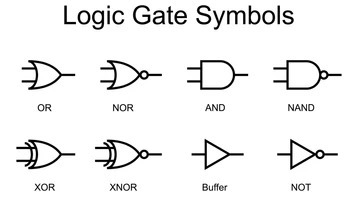
\includegraphics[width=300px]{images/logicGates.jpg}
\end{center}

\subsection{PLA (Programmable Logic Array)}
La PLA è una struttura formata da un barriera di AND (mintermini) e una barriera di OR.\\
Le funzione logiche hanno un costo rappresentato dal numero di porte e ingressi nella rete. 
Il costo può essere ridotto tramite metodi di tipo sistematico o grafico e si riuniscono sotto la "sintesi logica" 

\newpage
\subsection{Reti sequenziali}
Generalmente discutiamo di reti logiche dove in un istante viene dato un output, e nell'istante successivo
quell'output fa parte dei parametri in input. Ma dato che  i segnali richiedono tempo per propagarsi, questo
può causare errori, allora si utilizza il clock per temporizzare le azioni.\\
L'elemento base di memoria è chiamato \textbf{latch} (è composto da due porte NOR). I latch temporizzati vengono chiamati
\textbf{gated latch}. quest'ultimi sono controllati tramite 2 AND sugli ingressi di set e reset 

\begin{center}
  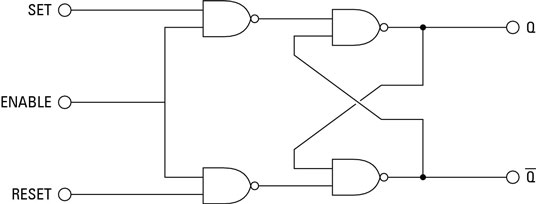
\includegraphics[width=250px]{images/gatedLatch.jpg}
\end{center}

I latch però soffrono l'inconveniente di poter ricevere un 1 sia in set che in reset. Per risolvere il problema del 
doppio 1 si usufruisce dei latch-D e flip flop:\\
il \textbf{latch-D} riceve S e R da un unica variabile messa in NOT su R, mentre il \textbf{flip-flop} usufruisce
di due latch e della negazione del clock, andando a separare nel tempo gli input

Questi elementi di memorizzazione strutturano i registri, cioé una serie di latch in grado di memorizzare una
\textbf{word di dati}. Il loro funzionamento avviene al fronte in salita del clock. Questi funzionamenti in base 
al clock vengono definiti come \textbf{edge triggered}, e offrono il vantaggio di rimuovere le situazioni di corse.

\newpage
\section{Assembly}
un programma in assembly è composto da una lista di istruzioni sequenziali con salti. Queste istruzioni si riuniscono
in 3 macrogruppi:
\begin{itemize}
  \item fetch: preleva un'istruzione dalla memoria
  \item decode: decodifica l'istruzione
  \item execute: eseguisce l'istruzione
\end{itemize}

Le istruzioni vengono anche categorizzate come:
\begin{itemize}
  \item operazioni aritmetico logiche
  \item movimenti di dati/assegnazioni di valore
  \item controlli di flusso
\end{itemize}

I dati con la quale lavoriamo sono classificati come \textbf{immediati} (constanti), \textbf{contenuti in registri}
(general purpose/specializzato, da 4 a 64) e \textbf{contenuti in memoria}

Infine, ci sono due tipi di architettura per la gestione dell processore: il \textbf{CISC} e il \textbf{RISC}

\subsection{RISC (Reduced Instruction Set Computer)}
Il RISC è un'architetture volta alla semplificazione dell'implementazione della cpu. Degli esempi di quest'
archittettura sono intel e RISC-V

I comandi per le istruzioni aritmentico-logiche segue il formato $\langle opcode\rangle\ 
\langle dst\rangle, \langle arg1\rangle, \langle arg2\rangle$\\
Mentre per l'accesso alla memoria la sintassi è:
\begin{itemize}
  \item load $\langle reg\rangle,\ \langle mem\ loc\rangle$
  \item store $\langle mem\ loc\rangle,\ \langle reg\rangle$
\end{itemize}



\subsection{CISC (Complex Instruction Set Computer)} 
Quest'architettura si concentra nel semplificare la scrittura dei programmi da parte del programmatore.
Il numero di istruzioni è maggiore, le istruzioni aritmetico logiche hanno operandi e destinazioni in 
memoria, e la sintassi risulta meno regolare.
Un esempio di questa architettura è ARM


\section{Assembly Risc-v}
Adesso esamineremo l'IS (Instruction Set) di RISC-V, un'architettura moderna e open source

\subsection{istruzioni aritmentico logiche}
\begin{quote}
  \center principio di progettazione n.1: 

  la semplicità favorisce la regolarità
\end{quote}

RISC-V prevede soltato istruzioni aritmentiche a 3 operandi:
\marginpar{commenti con \# }
\begin{center}
  a = b + c + d\\
  $\Downarrow$\\
  add a, b, c\\
  add a, a, d\\
\end{center}

Le istruzioni più complicate vanno suddivise in comandi più semplici:
\begin{center}
  a = (b+c)-(d+e)\\
  $\Downarrow$\\
  add t1, b, c \\
  add t2, d, e \\
  sub a, t1, t2\\
\end{center}  
In RISC-V però, gli operandi sono vincolati ad essere registri

\subsubsection{Registri}
\begin{quote}
  \center principio di progettazione n.2:
  
  minori sono le dimensioni, maggiore la velocità
\end{quote}
Operare solo tra registri semplifica e velocizza il progetto dell'hardware. 
Risc-v contiene \textbf{32 registri a 64 bit}, in maniera da ridurre la propagazione dei segnali 
all'interno del processore. Quindi, correggendo l'esempio di prima:
\begin{center}
  a = (b+c)-(d+e)\\
  $\Downarrow$\\
  add x5, x20, x21 \\
  add x6, x22, x23\\
  sub x19, x5, x6\\
\end{center} 
dove a = x19, b = x20, c = x21, d = x22, e = x23, t1 = x5 e t2 = x6.

\subsection{La memoria}
Ovviamente però il numero di registri non basta, per questo vengono usate istruzioni di 
trasferimento dai registri alla memoria (\textbf{store}) e dalla memoria ai registri
(\textbf{load}) 

Il caricamento e scaricamento di dati nei registri viene definito register spilling

Le costanti vengono memorizzate in un indirizzo. Questo metodo però risulta inefficente, quindi vengono usati gli operandi
immediati:\\
f = f + 4 => addi x22, x22, 4

\subsection{I numeri}

I numeri in Risc-V vengono rappresentati in esadecimale, in questo modo due cifre rappresentano un byte,
e una word con 8 cifre (es: 0xEA01BD1C). Una word viene quindi caratterizzata dall'ordine di lettura dei 
byte più o meno significativi. Se si parte dal byte meno significativo e si sale la denoteremo little endian,
se invece si parte da byte più significativo e si segnade, parliamo di big endian. Il little endian viene
utilizzato in intel e RISC-V, mentre il big endian da motorola e protocolli internet
RISC-V dedica un registro ad hoc (x0) alla costante 0

Le istruzioni in Risc-V vengono convertite in codici numerici univoci a 32 bit
\begin{itemize}
  \item primo (7bit), quarto (3bit) e sesto (7bit) codificano l'istruzione
  \item secondo (5 bit) : secondo operando
  \item terzo (5 bit): primo operando 
  \item quinto (5 bit): risultato
\end{itemize}
\begin{center}
  \begin{tabular}{c|c|c|c|c|c}
    funz7&rs2&rs1& funz3 & rd & codop 
  \end{tabular}
\end{center}
codop: codice operativo dell’istruzione
funz7 efunz3: codici operativi aggiuntivi
rs1: primo operando sorgente
rs2: secondo operando sorgente
rd: operando destinazione

Trade-off 
\begin{quote}
  \center principio di progettazione n.3: 

  un buon progetto richiede buoni compromessi
\end{quote}


RISC-V con le sue istruzioni a 32 bit limita il numero di istruzioni, di registri e di modalità d'indirizzamento,
ma ci guadagna in efficenza

\subsection{Operazioni logiche}
RISC-V offre varie funzioni per operare su porzioni di words o su singolo bit:

\textbf{Shift logico}\\
si usa per inserire degli zeri nella posizione meno (shift a sinistra) o più (shift a destra)significativa 
Lo shift a destra però, può generare degli overflow. Per risolvere questo problema si utilizza lo shift aritmentico
(srai) che, invece di aggiungere bit pari a 0, si aggiungono bit pari al bit di segno

\newpage
altre operazioni logiche sono:

\textbf{AND bit a bit}\\ la word salvata tiene valori a 1 solamente se erano a 1 in entrambe le word confrontate

\textbf{OR bit a bit}\\ la word salvata tiene il valore a 1 se compare almeno una volta nelle word confrontate

\textbf{OR esclusivo (XOR)}\\mantiene il bit a 1 solamente se i due bit confrontati sono differenti.
Viene, per esempio, usato per resettare un registro (xor x9, x9, x9)

\textbf{NOT}\\
il not è un'operatore unario e di conseguenza non è supportato da RISC-V, ma si può ottenerlo
attraverso un XOR: NOT A $\rightarrow$ XOR (A, 1)

\textbf{istruzioni con condizioni}\\
nelle architetture le condizioni si convertono in istruzioni di salto condizionato. Queste istruzioni si
caratterizzano in due tipi:
\begin{itemize}
  \item per uguaglianza: beq rs1, rs2, L1 $\rightarrow$ se rs1 è uguale a rs2 allora salta all'etichetta L1
  \item per differenza: bne rs1, rs2, L1 $\rightarrow$ se rs1 è diverso a rs2 allora salta all'etichetta L1
\end{itemize}

es:\\
costrutto if: if(i==j) f=g+h; else f=g-h;

\begin{tabular}{l l}
     &bne x22, x23, ELSE \\
     &   add x19, x20, x21   \\
     &  beq x0, x0, ESCI\\
ELSE:& sub x19, x20, x21\\
ESCI:&
\end{tabular}

\newpage

\textbf{Cicli}
sfruttando i salti condizionati si possono creare dei cicli, per esempio:

\begin{tabular}{l l}
Ciclo: &slli x10, x22, 3\\
       &add x10, x10, x25\\
       &ld x9, 0(x10)\\
       &bne x9, x24, Esci\\   
       &addi x22, x22, 1\\
       &beq x0, x0, Ciclo\\
Esci:  &...
\end{tabular}

Alcune considerazioni:\\
le istruzioni tra 2 salti condizionati (conditional branch) vengono chiamati blocchi di base.
L'individuazione di questi blocchi è una delle prime fasi della compilazione.

ulteriori istruzioni di salto sono $blt$(salta se minore),bge (salta se maggiore o uguale),
bltu e bgeu (blt e bge ma unsigned). Le versioni unsigned semplicemente tengono conto
o meno del bit significativo

\textbf{costrutto switch}\\
Memorizza i vari codici da eseguire in una tabella, per poi caricare in un registro 
l'indirizzo del codice da eseguire.

infine abbiamo l'istruzione di salto jalr che salta all'indirizzo contenuto nel registro

\newpage
\subsection{Procedure}
Le funzioni (o procedure) svolgono un ruolo fondamentale,ma necessitiamo di un protocollo
per richiamarle. Un protocollo necessità di standardizzare
\begin{enumerate}
  \item dei posti noti dove caricare i parametri in input
  \item il trasferimento del controllo alla procedura
  \subitem aquisizione dei parametri in input
  \subitem esecuzione della procedura
  \subitem caricamento dei valori di ritorno in posti noti
  \subitem restituzione del controllo al chiamante
  \item la raccolta dei valori di ritorno e la pulizia delle tracce della procedura
\end{enumerate}
RISC-V affronta questo meccanismo usando il più possibile i registri attraverso delle convenzioni:
\begin{itemize}
  \item x10-x17: usato per parametri in ingresso e valori di ritorno
  \item x1: indirizzo di ritorno
  \subitem questo indirizzo viene usato particolarmente per istruzioni di jump and link (jal), che effettuano il salto
  e memorizzano in x1 l'indirizzo di ritorno
  \subitem alla fine della procedura sarà sufficiente fare un salto (jalr x0, 0(x1))
\end{itemize}
nel caso i registri non bastino viene usato lo stack x2, chiamato anche \textbf{sp} (Stack Pointer). Alla fine della procedura è importante
ricordare di pulire lo stack

\begin{itemize}
  \item  x5-x7 e x28-x31 sono registri temporanei
  \item  x8-x9 e x18-x27 sono registri in cui salvare il contenuto in caso di chiamata a procedura
\end{itemize}

In caso di variabili locali e procedure annidate la gestione dei registri può diventare complessa
Questo viene risolto usando lo stack per allocare variabili locali e valori del registro di ritorno x1

\textbf{Storage class}
le variabili in C sono associate a locazioni di memoria caratterizzate per tipo e storage class. Il C ha due tipi
di storage class: Automatic (le variabili locali) e Static. Le variabili static vengono memorizzate da RISC-V
nel registro $x3$, chiamato anche \textbf{gp} (global pointer). Per quello che riguarda le automatic, esse sono memorizzate
nei registri o nello stack in caso i registri non bastassero

\textbf{record di attivazione}
Il segmento di stack che contiene variabili locali e i registri salvati è chiamato record di attivazione
(o stack frame). Le variabili locali sono individuate tramite un offset. In alcuni casi il registro
sp può essere scomodo, percui in alcuni programmi viene usato il registro x8 come \textbf{fp} o frame pointer,
come puntatore alla prima parola doppia del frame della procedura

per tutti le variabili allocate dinamicamente, RISC-V procede per indirizzi crescenti

Riassunto convenzione sui registri:
\begin{center}
  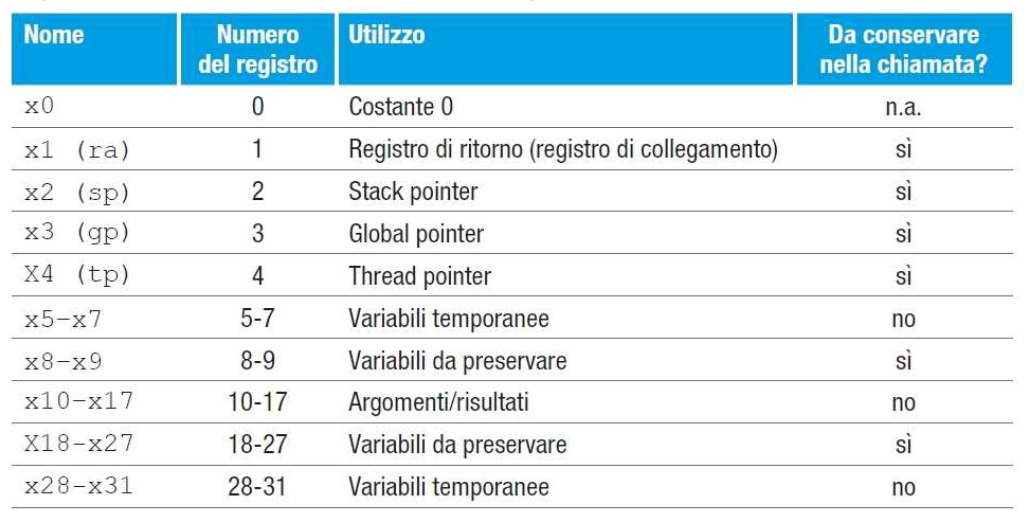
\includegraphics[width=350px]{images/RISC-V_RegisterConvention.jpeg}
\end{center}


%(elaborazione)
%spesso la ricorsione può essere inefficente, conviene piuttosto generare una ricorsione 
%"di coda", cioé che tiene conto del procedimento e ritorna direttamente il risultato

%(Ottimizzazione)
%alcuni compilatori sanno riconoscere la ricorsione di coda. Le caratteristiche
%principali sono: il chiamante ritrna subito dopo la jalr, x5 e gli altri registri non cambiano,
%il chiamato protrebbe direttamente ritornare al ra del chiamante...
%gcc fa questo con opportuni flag 

\newpage
\section{Intel}

Intel è un'archittettura di tipo CISC usata in laptop, desktop e servers. Possiede diverse modalità di
funzionamento e diversi assembler. Nel nostro caso useremo GNU

\subsection{Registri}
Intel usa 16 registri general purpouse a 64 bit caratterizzati dal prefisso \%. Alcuni dei più importanti
sono:
\begin{itemize}
  \item \%rsp: stack pointer
  \item \%sbp: base pointer
  \item \%rsi e \%rdi: registri source e destination per la copia di Array
  \item \%rip: Instruction pointer
  \item \%rflags: estende \%flags, che contiene flag come CF (flag di carry), ZF(risultato 0),
  SF(risultato negativo), OF(flag di overflow). Questi registri speciali vengono usati da
  istruzioni di salto condizionale
\end{itemize}

\subsection{Convenzioni di chiamata}
Le chiamate in Intel sono molteplici, e cambiano in base alle specifiche tecniche dell'ABI. Alcune però sono 
comuni a tutte le CPU:
\begin{itemize}
  \item i primi 6 argomenti sono in \%rdi, \%rsi, \%rdx, \%rcx, \%r8 ed \%r9, mentre gli altri vengono impilati nello stack
  \item i valori di ritorno stanno in \%rax e \%rdx
  \item i registri vengono preservati \%rbp, \%rbx, \%r12, \%r13, \%r14 ed \%r15
  \item i valori di ritorno in \%rax e \%rdx
\end{itemize}


\subsection{Indirizzamento}
Con intel le istruzioni sono principalmente a 2 operandi con destinazione implicita. Per la sorgente si usano
operandi immediati(\$20), registri (\%rax), o indirizzi di memoria (0x0100A8). Per le destinazioni sono utilizzabili.
L'accesso alla memoria avviene seguendo la seguente sintassi:

$\langle displ\rangle$ ($\langle base reg\rangle, \langle index reg\rangle, \langle scale\rangle$)

 - $\langle displacement\rangle$: costante a 8, 16 o 32bit\\
 - $\langle base\rangle$: valore in registro \\
 - $\langle indice\rangle$: valore in registro \\
 - $\langle scala\rangle$: valore costante

In casi speciali scala, indice, base e displacement possono essere omessi

\subsection{Istruzioni intel}
Le istruzioni Intel sono molte, inutile sarebbe elencarle tutte, ma condividono una sintassi comune:

$\langle opcode\rangle \langle source\rangle, \langle destination\rangle$

Il parametro $\langle opcode\rangle$ può terminare con b/w/l/q per indicare che l'operazione viene 
effettuata su 8/16/32/64bit

\newpage
\textbf{istruzioni comuni}
\begin{itemize}
  \item istruzioni logico aritmentiche
  \subitem mov, add, sub, mul, div, inc/dec (incrementa/decrementa di 1), 
  \subitem rcl/rcr/rol/ror (rotate)
  \subitem sal/sar/shl/shr (shift aritmentici e logici)
  \subitem and, or, xor, not, neg(complemento a 2, negazione), nop.
  \item push/pop: inserisce/rimuove dati nello stack
  \item cmp/test: comparano i 2 argomenti e settano i flag nel flag register
  \item jmp, je/jnz/jc/jnc: salti condizionati
  \item call/ret: chiamata/ritorno alla procedura
  \item lea (Load effective address) è un istruzione utilizzata per calcolare indirizzi:
  \subitem calcola e e memorizza l'indirizzo senza caricare nulla dalla memoria
  \subitem viene anche usato per fare somme
\end{itemize}
 

\newpage
\section{ARM}
L'archittettura ARM (o Advanced Risc Machine) è usata nei sistemi embedded e in smartphone e tablet. È caratterizzato
dall'utilizzo di 16 registri e modalità d'indirizzamento potenti. 

NB: ARM è una famiglia di CPU, con ISA differenti ma simili fra loro 

\subsection{Registri}
I 16 registri a 32 bit, r0-r15, sono quasi tutti general purpouse (eccezion fatta per r15). Alcuni registri sono
muniti di sinonimi: r13=sp(stack pointer) e r14=lr(link register). Il registro r15 contiene il PC e i flag 
che sono contenuti negli ultimi 4 bit.
 
\subsection{Convenzioni di chiamata}
Le convenzioni di chiamata non fanno parte dell'archittettura, ma le varie ABI condividono determinati elementi

I registri r0-r3 sono registri temporanei non preservati, nel caso ci siano più di 4 argomenti viene usato lo stack.
I registri r4-r11 invece vengono preservati, e i valori di ritorno vengono immagazzinati in r0-r1



\subsection{Indirizzamento}
Le istruzioni generalemente usufruiscono di 3 argomenti:l'identificatore dell'istruzione, l'operando sinistro (registro)
, operando destro(immediato o registro). L'accesso alla memoria avviene tramite le istruzioni ldr/str 
(load register/store register) e ldm/stm (load/store multiple).\\Gli operandi in memoria vengono indirizzati tramite
una base più un offset (immediato) o indice.




\newpage
\rightline{Nona settimana}
\section{Toolchain}
La CPU funziona con un linguaggio di basso livello composto, da 1 e 0, troppo complesso da programmare. La conversione
viene eseguita dal compilatore

\subsection{Esempio: il compilatore di C}
la compilazione del linguaggio C segue i seguenti passaggi:
\begin{enumerate}
  \item Preprocessore: gestisce le direttive di sostituzione del codice
  \item Compilatore: da C ad assembly 
  \item Assembler: da assembly a linguaggio macchina
  \item Linker: unisce linguaggio macchina con le librerie per creare un eseguibile
\end{enumerate}
Questo processo è gestito automaticamente da un Driver

\textbf{gcc} (Gnu Compiler Collection)\\ È in grado di compilare vari linguaggi in assembly per varie CPU. Per 
operare utilizza vari programmi: cpp,cc,as e ld 

\textbf{Da C ad Assembly}\\ dato un file .c, il comando gcc -S invoca cc per generare un file assembly .s.
cc riconosce l'archittettura dulla CPU, applica vari livelli di ottimizzazione (tramite l'opzione -o)

\textbf{Da Assembly a linguaggio macchina}\\ Usando gcc -c viene invocato cc e successivamente as, per generare un
file .o, o file oggetto. as non solo converte i codici memonici in sequenze di bit, ma converte pseudo-istruzioni,
i numeri da decimale/esadecimale a binario, genera metadati e gestisce label e salti.\\
Con pseudo-istruzioni si intendo le istruzioni non di tipo nativo, che sono formate da altre istruzioni macchina
e che esistono per semplificare la programmazione.

\newpage
\textbf{File oggetto}\\ È composto da segmenti distinti:
\begin{itemize}
  \item header: specifica dimensione e posizione degli altri segmenti del file oggetto
  \item text segment: contiene il codice in linguaggio macchina
  \item data segment: contiene tutti i dati statici e dinamici allocati
  \item symbol table: associa simboli a indirizzi e enumera quelli non definiti
  \item relocation table: enumera istruzioni e dati che dipendono da indirizzi assoluti, o definiti 
  quando il programma viene caricato in memoria
  \item altro...
\end{itemize}

\textbf{Da file oggetto a eseguibile}\\ Il passo finale, tramite gcc senza opzioni, richiama il linker ld, che decide
la disposizione di codice e dati nella memoria, associa indirizzi assoluti a tutti i simboli, risolve i siboli 
lasciati indefiniti nel file .o e sistema la tabella di rilocazione. In breve, ld rimuove le tabelle dei simboli  e 
di rilocazione, generando codice macchina con riferimenti corretti.\\
Un linker gestisce vari tipi di simboli:
\begin{itemize}
  \item simboli definiti: associati a un indirizzo nella tabella dei simboli
  \item simboli non definiti: usati in un file, ma definiti in un file diverso. Se il linker, cercando in altri file 
  non trova il simbolo, da errore di linking
  \item simboli locali:  definiti e usati in un file, ma non usabile in altri file
\end{itemize}
in tre passi, il linking consiste nel: disporre in memoria i vari segmenti dei file .o, assegnare un indirizzo assoluto
ad ogni simbolo contenuto nelle tabelle e correggere le istruzioni delle tabelle di rilocazione con degli indirizzi 
calcolati. Il risultato viene poi incapsulato in un file eseguibile (segmenti, informazioni per il carimento in memoria,
altri dati)

\subsection{Librerie}
il compilatore, o il sistema, fornisce delle funzioni predefinite. Queste funzioni sono contenute in librerie, o collezioni
di file .o. Le librerie sono di due tipi: statiche (.a) e dinamiche (.so)

\textbf{Librerie statiche}\\ ld inserisce tutto il codice della libreria nell'eseguibile. Quest'ultima serve solo 
durante il linking. 

\textbf{Librerie dinamiche}\\ ld inserisce un riferimento a un linker dinamico (es: /lib/ld-linux.so) alla libreria,
senza includerla nell'eseguibile. All'esecuzione del programma, il linker viene caricato ed eseguito, caricando le 
librerie e l'eseguibile, facendo il linking.

La differenza principale tra librerie statiche e dinamiche sta nelle dimensioni e nella complessità di caricamento
del programma da parte del SO. Un'altro vantaggio delle librerie dinamiche rispetto a quelle statiche è che dato che 
le librerie non sono caricate, permette di aggiornarle senza dover ricompilare l'eseguibile.

\textbf{Lazy linking}\\ Può capitare che alcune librerie vengano poco usate a tempo di runtime, quindi, invece che
linkare la vera funzione, può essere chiamato uno stub, che esegue caricamento, rilocazione e linking solo quando 
necessario

(es: slide 18, toolchain)

\newpage
\section{Il processore}

panoramica
- nell'esecuzione delle istruzioni, ci sono due fasi iniziali comuni
 - prelievo dell'istruzione dalla memoria
 - lettura dei registri
- i passi sccessivi sono simili, ma dipendono dall'istruzione

-le istruzioni più comuni usano la alu 
 - calcolo dell'indirizzo per l'accesso alla memoria
 - istruzioni aritmentico logiche
 - confrontare le condizioni per eseguire dei salti
- successivamente le tre classi divergono
 - le istruzioni d'accesso alla memoria salvano il dato in memoria
 - le istruzioni aritmetico logiche memorizzano il risultato nel registro
 - le istruzioni di salto cambiano il valore del registro PC in base al confronto

Il processore utilizza anche i multiplexer per effettuare decisioni. Per esempio le istruzioni
possono provenire dal banco dei registri o dal codice dell'istruzione stessa, per selezionare
i due tipi, viene usato un multiplexer. Oppure per far decidere alla ALU che operazione effettuare,
dai banchi dei registri per decidere in quale registro scrivere o dalla memoria dati per determinare
se vogliamo leggere o scrivere. Per decidere come utilizzare i vari ingressi di controllo viene 
utilizzata un'unità specifica.

figura slide 10

\subsection{Reti logiche}
una rete logica combinatoria consiste in un circuito di porte logiche dove l'output è una funzione statica dell'input.
Contiene anche elementi di stato, cioé registri, memorie dati e memorie d'istruzioni. Questi elementi di stato sono detti 
sequenziali perché l'uscita a un ingresso dipende dagli ingressi precendenti. 

\textbf{Flip-flop}\\ L'elemento base per la memorizzazione dei bit è il flip-flop D-latch. Un array di latch forma Un
registro. Un latch viene definito come asserito o non asserito in base al livello logico che possiede

\subsection{Temporizzazione}
La temporizzazione è la metodologia che determina quando i segnali possono essere letti o scritti in base al ciclo di clock.
La più utilizzata è quella dei fronti, cioé della salita o discesa dei fronti di clock.

\subsection{Data path}
\begin{center}
  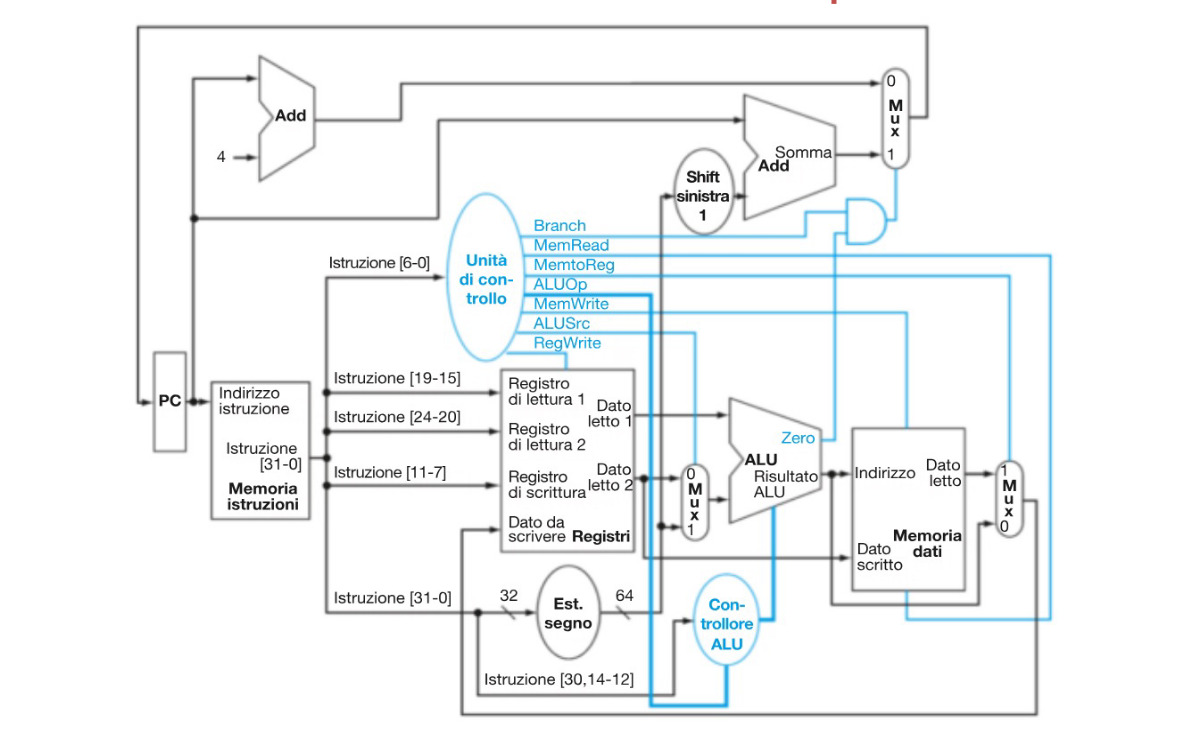
\includegraphics[width=400px]{images/CPU_Structure.jpeg}
\end{center}

\textbf{Memoria istruzioni}\\ memoria che contiene le istruzioni

\textbf{Program Counter}\\Registro che contiene l'indirizzo dell'istruzione da caricare

\textbf{Sommatore (ALU)}\\ALU specializzata per incrementare in PC

\textbf{ALU}\\Effettua calcoli e confronti, a un parametro di uscita speciale che viene impostato a 1 quando da un confronto
risulta che i due elementi sono uguali

\textbf{Controllore ALU}\\La ALU viene controllata tramite dei bit di controllo generati da questa unita. Questi bit
sono determinati dai campi funz3, funz7 e dai due bit ALUop. I bit ALUop sono definiti dall'unità di controllo

\textbf{Banco dei registri}\\prende in entrata i registri dove leggere/scrivere e il dato da scrivere, e in uscita rida i 
dati letti

\textbf{Unità di memoria dati}\\Questa memoria si differisce dalla memoria istruzioni per la capacità di operare sia 
in lettura che in scrittura

\textbf{Unità di estensione del segno}\\viene utilizzata per estendere il campo a 12bit a 64bit per applicare l'offset
usato nei salti condizionali

\textbf{RegWrite}\\Se abilitato scrive nel registro specificato il dato in ingresso

\textbf{ALUSrc}\\Applica un'estensione del segno al secondo operando della ALU

\textbf{PCSrc}\\Applica un'estensione del segno per effettuare dei salti nelle istruzioni contenute nel PCSrc

\textbf{MemRead/MemWrite}\\Determina il tipo di interazione con la memoria dati

\textbf{MemtoReg}\\Determina se il dato inviato al register file provenga dalla ALU o dalla memoria

\textbf{Branch}\\Interagisce con il segnale di zero proveniente dalla ALU per effettuare un salto a istruzione

\textbf{Unità di controllo}\\È una componente che genera tutti i segnali di controllo in base al codice operativo
dell'istruzione ricevuta da PC. I segnali con la quale interagisce sono ALUSrc, MemtoReg, RegWrite, MemRead, 
MemWrite, Branch, ALUOp1, ALUOp0

\newpage
\section{Pipeline}
Il ciclo di clock è definito dalle istruzioni più lente, per esempio quelle di accesso alla memoria. Per ottimizzare
i tempi di inattivita vengono implementate le pipelines, che permettono la paralelizzazione dei processi. 
Generalmente il miglioramente viene calcolato come:
\begin{center}
  $tempo\ tra\ due\ istruzioni\ con\ pipeline\ =\ \frac{Tempo\ senza\ pipeline}{Numero\ di\ stadi}$
\end{center}
Dove con stati intendiamo le diverse fasi che compongono un'istruzione.\\In realtà questa regola non si può
applicare perfettamente a causa della durata di alcune istruzione. In generale il miglioramento è inferiore 
rispetto a quello calcolato tramite la formula.

\subsection{Pipelines e architetture RISC}
L'architettura RISC offre dei vantaggi specifici che migliorano l'implementazione delle pipelines:
\begin{itemize}
  \item Tutte le istruzioni hanno la stessa lunghezza, con conseguente prelievo più efficente
  \item i codici degli operandi sono in posizione fissa. Questo permette la lettura del register file in 
  parallelo con la decodifica dell'istruzione
  \item gli operandi in memoria sono disponibili solo per ld e sd. Questo permette il calcolo degli indirizzi in ALU
  \item gli accessi allineati permettono un solo ciclo di trasferimento per gli accessi in memoria
\end{itemize}

\newpage
\subsection{Hazard}
A causa del loro funzionamento, alcune istruzioni non possono essere eseguiti in un solo ciclo di clock. Le 
condizioni che si generano vengono definite \textit{hazard} e possono essere di diverse tipologie

\subsubsection{Hazard strutturali}
L'hazard strutturale è una condizione dove l'archittettura stessa del processore rende impossibile l'esecuzione 
di alcune istruzioni in pipeline. Per esempio, con una sola memoria non è possibile sia caricare che prelevare 
operandi nello stesso ciclo di clock.

\subsubsection{Hazard sui dati}
Questa condizione si verifica quando un'istruzione necessità di dati provenienti da un'istruzione precedente. 
quindi il processore deve fermare l'istruzione ed attendere finche il necessario dato non viene salvato
nell'istruzione precedente. In alcuni casi il compilatore è in grado di effettuare alcune ottimizzazioni per 
ottenere quel risultato. Una di queste ottimizzazioni è \textit{l'operation forwarding}. Nel caso abbiamo due 
istruzioni algebriche nel quale il risultato della prima è operando della seconda, l'operation forwarding salta 
la parte di scrittura nel registro del risultato, e lo reinserisce direttamente nella ALU. 

\subsubsection{Hazard sul controllo}
Quando viene effettuato un salto condizionato, c'è bisogno di attendere il risultato del controllo (o della 
condizione del salto) per determinare qual'è l'istruzione successiva da caricare. Questo tempo di attesa è un 
hazard di controllo. Maggiore è il numero di stadi di un'istruzione, maggiore è il ritardo sulla pipeline.\\
Per risolvere questo hazard vengono usufruiti vari metodi per la previsione del salto. Uno di questi consiste
nel caricamento dell'istruzione successiva, e nel caso le condizioni di salto siano positive, l'istruzione viene
abortita dalla pipeline e sostituita con quelle espressa nel salto. Questo non è il metodo più efficente, infatti
esistono circuiterie più complesse che permettono di memorizzare l'esito del branch e mantenere un comportamento
coerente

\newpage
\section{Gerarchia di memoria}
\subsection{Terminologia}
\textbf{Memoria indirizzata direttamente}\\Di tipo volatile, è limitata dallo spazio di indirizzamento del processore
e accessibile in qualsiasi momento nella memoria principale

\textbf{Memoria indirizzata indirettamente}\\Di tipo permanete, possiede uno spazio di indirizzamento di tipo 
software. Generalmente è il sistema operativo a gestire il passaggio tra memoria principale e periferica

\textbf{Tempo di accesso}\\Tempo richiesto per una operazione in lettura o scrittura

\textbf{Tempo di ciclo}\\Il tempo dell'intervallo tra due operazioni consecutive

\textbf{Accesso casuale}\\I dati non sono ne in ordine ne condividono alcuna relazione. Accesso tipico di memorie a
semiconduttori

\textbf{Accesso sequenziale}\\L'accesso alla memoria è ordinato o semi-ordinato. Il tempo d'accesso dipende dalla
posizione

\textbf{RAM (Random Access Memory)}\\Memoria in lettura/scrittura a semiconduttori

\textbf{ROM (Read Only Memory)}\\Memoria a semiconduttori in sola lettura

\subsection{Tipi di memoria}
\subsubsection{Memorie RAM}
Le RAM memorizzano singoli bit in byte e/o word. Può supportare il parallelismo della capacità (128K $\times4$),
questo influenza il numero di pin I/O

\subsubsection{Memorie statiche (SRAM)}
In questo tipo di memoria, i bit possono essere tenuti indefinitamente, finche è presente l'alimentazione. Sono 
estremamente veloci e consumano poca corrente, il tutto a un costo maggiore.

Sono formate da una linea word che determina l'appertura di due interruttori $T_{1}$ e $T_{2}$ che isolano 
un latch. Infine il dato viene trasmesso tramite due linee $d$ e $d^{I}$, dove $d^{I}=NOT(d)$

\subsubsection{RAM Dinamiche (DRAM)}
Economiche e a alta densità, mantengono la carica attraverso un codensatore. Necessitano di un \textit{refresh}
continuo per mantenere il dato, il che aumenta i consumi.

È formata da un interruttore che chiude il circuito a un condensatore, da due linee di word e di bit e un \textit{
sense amplifier}, cioé un circuito che mantiene la tensione sul condensatore. Il sense aplifier viene attivato a 
ogni ciclo di lettura, quindi il chip di memoria contiene un circuito per una lettura periodica di tutta la memoria

Dato che le DRAM sono molto capienti, le celle sono suddivise in righe e colonne, e i loro pin per I/O vengono 
gestiti in modo da trasmettere sugli stessi pin sia gli indirizzi di riga e colonna. Questa divisione in righe e
colonne viene riferita attraverso byte.

Il trasferimento di dati avviene in blocchi. Per ottimizzare il processo, si evita di riselezionare la riga ad ogni
accesso. Questo metodo è chiamato Fast Page Mode (FPM)

Le DRAM vengono definite asincrone dato che l'accesso viene definito dai segnali RAS e CAS. Per questo vengono aggiunti
dei buffer che caricano i dati per poi essere usati dalla CPU ad ogni giro di clock

\textbf{Terminologia:}\\Latenza: tempo di accesso a una parola\\Velocità/banda: velocità di trasferimento in FPM

\subsubsection{Double Data Rate SDRAM}
Le DDR-SDRAM sono delle memorie sincrone che trasferiscono dati sia sul fronte positivo che negativo di clock. I
dati pari e dispari sono organizzati in due banchi di memoria. Questa tecnica mantiene la stessa latenza raddopiando 
la banda.

\subsection{Gerarchia di memoria}
Le memorie, come visto, hanno velocità e capacità diverse. Per ottenerle entrambe si danno al processore l'illusione 
di avere una memoria veloce e estesa spostando dati tra tipi di memoria in base a due metodi di utilizzo:

\textbf{Località temporale}\\
Quando viene usata una locazione di memoria, è probabile che venga riutilizzata in poco tempo

\textbf{Località spaziale}\\
Quando viene usata una locazione di memoria, è probabile che vengano usate le locazioni vicine

Questi dati vengono spostati fra vari livelli di memoria più (livelli alti) o meno (livelli bassi) vicini al
processore.

\subsubsection{Terminologia}
\textbf{Blocco:} unità di informazione

\textbf{Hit Rate:} Frazione degli accessi in cui trovo i dati al livello superiore

\textbf{Miss Rate:} frazione degli accessi in cui non trovo i dati al livello superiore

\textbf{Tempo di hit:} tempo necessario per accedere a un dato trovato al livello superiore

\textbf{Penalità di miss:} tempo necessario per accedere a un dato non trovato al livello superiore

\subsubsection{Cache}
La cache è una locazione di memoria completamente trasparente al programmatore dove vengono riposti alcuni dati.
Per determinare un indirizzo di memoria a uno di cache, viene usata la mappatura diretta, cioé ad ogni indirizzo 
della memoria corrisponde un indirizzo preciso nella cache. Per determinare la presenza di un determinato dato viene 
usato un \textit{tag} (che contiene una parte del dato sufficente a effettuare il riconoscimento, generalemente i 
bit più significativi) e un bit di validità

L'indirizzo di un blocco viene dato da $\frac{indirizzo\ del\ dato}{byte\ per\ blocco}$ e identificato come 
(indirizzo blocco) modulo (numeri blocchi nella cache)

\textbf{Trade-off}
I blocchi di cache di grandi dimensioni riducono la probabilità di miss ma diminuisce l'efficacia della località
temporale e aumenta il costo di gestione (o spostamento di byte)

\textbf{Gestione delle miss}
In caso di miss viene generato uno stallo nella pipeline per gestire il trasferimento di dati dalla memoria principale
alla cache.

Le scritture vengono gestite con la stessa logica per garantire la consistenza dei dati. Il \textit{Write-through}
è una politica di gestione che scrive in memoria principale indipendemente dalla presenza di hit o miss. In 
alternativa c'è il \textit{Write back}, cioé le scritture avvengono in cache e l'update in memoria principale avviene
solo con il rimpiazzamento del blocco o accesso da parte di un altro core

\subsubsection{Cache associative}
Le cache con mappatura diretta generano miss quando delle locazioni di memoria si mappano sullo stesso blocco. Perciò
vengono usate le cache associative.\\Le cache \textit{completamente associative } usano l'intero indirizzo di blocco come tag. 
Per una ricerca efficente bisogna usare n compattatori pari al numero di blocchi da processare in parallelo. Questo è
parecchio costoso in termine di hardware, perciò viene usato solo su cache molto piccole. In alternativa si usa la 
cache \textit{set-associativa}, che consiste in una cache dove un blocco di memoria è mappato su una linea contenente n
blocchi diversi. Sui blocchi facenti parte della linea viene effettuata una ricerca parallela

Per quello che riguarda gli indirizzi, nella mappatura set-associativa, indirizzo è dato da (indirizzo blocco) modulo 
(numero linee della cache)

Nelle cache associative, quando la linea è piena viene usata una politica di sostituzione su base FIFO o Least Recently 
Used (lettura)

\newpage
\section{I/O}
I dispositivi di I/O sono essenziali per il funzionamento di un calcolatore. Essi devono essere eterogenei ed 
espandibili, e rispettare prestazioni specifiche, in genere la latenza o il throughput.\\ I dispositivi sono collegati
al processore tramite un bus

\textbf{Classificazione}\\ I dispositivi I/O vengono classificati in base a comportamento, partner (uomo o macchina)
e velocità di trasferimento

\subsection{Bus}
Come accennato i bus si occupano di connettere il processore con i dispositivi I/O. Esistono due tipi di bus:
\begin{itemize}
  \item Bus processore/memoria: bus corti, ad alta velocità di trasmissione
  \item Bus I/O: bus lunghi che connettono periferiche eterogenee. Tipicamente non si connettono direttamente al 
  processore ma a un bus processore/memoria o a un bus di sistema
\end{itemize}

\textbf{Terminologia}
\begin{itemize}
  \item Transazione di I/O: invio indirizzo e spedizione/ricezione dati
  \item Input: trasferimento dati verso il processore
  \item Output: trasferimento dati dalla memoria verso il dispositivo
\end{itemize}

\subsubsection{Bus sincrono}
Le comunicazioni avvengono con un protocollo collegato al ciclo di clock. Questa tipologia è molto semplice da 
implementare e molto veloce, però risulta meno robusto al drift di clock, e in più tutte le periferiche devono 
andare a velocità di clock

\subsubsection{Bus asincrono}
In alternativa al bus sincrono si usa quello asincrono. Il suo funzionamento funziona su base di segnali chiamati 
\textit{handshake}. Questo permette una maggiore robustezza ai ritardi e rende le periferiche indipendenti dal clock
del processore. Come contro però risulta lento nelle interazioni e richiede una circuiteria più complessa

Nelle tecnologie odierne vengono usati dei bus ibridi, ma principalmente asincroni

\subsection{SO}
Un sistema operativo deve gestire i permessi di accesso a un dispositivo I/O, fornire comandi di alto livello per
gestire operazioni di basso livello, gestire le interruzioni generate dai dispositivi I/O e fornire l'accesso a un 
dispositivo ai vari programmi in maniera equa.\\Per supportare tutte queste funzioni il SO deve essere in grado di 
inviare comandi alle periferiche, permettere ai dispositivi di notificare una corretta esecuzione di un'operazione e
consentire trasferimenti diretti di dati tra dispositivo e memoria

\textbf{Comandi ai dispositivi}\\Questo avviene tramite determinate parole di controllo. L'implementazione di questo
meccanismo funziona tramite la scrittura/lettura in specifiche locazioni di memoria (memory mapped I/O) o tramite
alcune istruzioni speciali.\\ES:scrivendo una parola in una locazione associata al dispositivo, il sistema ignora la 
scrittura, mentre il controllore di I/O intercetta l'indirizzo e lo converte in comando al dispositivo.

\textbf{Trasmissione/Ricezione dati}\\Per la trasmissione viene usata la attesa attiva, o \textit{polling}, cioé 
viene inviato un comando di scrittura/lettura alla periferica e poi si entra in un ciclo di attesa fino a quando
il dato è pronto. Questo può essere applicabile quando le operazioni di I/O avvengono a una velocità predeterminata,
in altri casi il tempo di attesa diventa troppo dispendioso per il processore. Perciò viene usato l'I/O a interruzione
di programma (interrupt driven I/O).\\Un'interruzione I/O è un segnale usato per segnalare al processore che la 
periferica è pronta ad effettuare il trasferimento. Queste interruzioni sono sempre asincrone e possono avere vari 
gradi di urgenza. Il vantaggio di questo metodo è che l'interruzione arriva solamente quando il dato è pronto ad
essere trasferito in memoria, il tutto però richiede un hardware speciale in grado di generare e gestire le 
interruzioni. Per gestire queste interruzioni vengono generate delle eccezioni.

\newpage
\subsection{Eccezioni}
Un'eccezione è un trasferimento non programmato del controllo del programma. Il sistema per gestire delle eccezioni 
registra il punto di interruzione, salva lo stato e come riprendere il processo a eccezione finita. Esistono 3 tipi 
di eccezione:
\begin{itemize}
  \item Interrupts: causate da eventi esterni I/O, sono asincrone e possono essere gestite facilmente nello spazio
  tra due istruzioni
  \item Traps (eccezioni): causate da eventi interni al programma (condizioni eccezionali, errori e fault), sono 
  sincrone al programma e vengono gestite da un trap handler che riprova l'istruzione o abortisce il programma
  \item Environment call/break
\end{itemize}

Le eccezioni vengono gestite tramite un Exception Handler, che gestisce l'eccezione tramite vettore d'interruzione
o salto all'indirizzo della routine di gestione. In entrambi i casi però, l'exception handler deve preservare lo stato
della macchina.

\textbf{salto alla routine di gestione}\\Si effettua un salto nel PC a un indirizzo specifico, questo permette di
evitare di passare dalla memoria, ma richiede che nella routine di gestione venga analizzata la causa dell'eccezione

\textbf{Vettore d'interruzione}\\In una tabella vengono memorizzati gli indirizzi delle routine di gestione per ogni
possibile causa di eccezione. Questo metodo richiede però il passaggio in memoria per prelevare l'indirizzo della 
routine di gestione

Nel momento in cui viene generata un'eccezione, lo stato della macchina può essere salvato in stack, su registri 
ausiliari (più o meno visibili) o in registri speciali. In Risc-V vengono usati sia lo stack che dei registri 
speciali. Quest'ultimi in particolari sono situati in un banco interno al processore chiamato Control Status Register
(CSR)



\end{document}